\chapter{Synthesizing Data for Object Detection on \ac{MAV}}
\label{sec:training}

Machine learning relies on the assumption that a general concept can be extracted from a limited set of examples. 
In Supervised Machine Learning, the set of examples $X$ is augmented with a set of labels $Y$ that describes task dependent information that is present in the sample. By defining and optimizing a loss function $L$ the concept is extracted and represented by a hypothesis $h$. For the optimization procedure different models can be applied. They differ in model assumptions, as well as the amount of parameters that are optimized during training. 

The bias-variance trade-off relates the amount of annotated examples used for training and model complexity. It states that with a given amount of training examples, a more complex model might be able to improve in that particular training set, but it will therefore loose performance in other datasets (reduced bias). On the other hand a more simple model will maybe not capture the full information of the training set, but it will have a more stable performance across datasets (reduced variance). The only way to use a more complex model without increasing the variance is to increase the amount of training data.

In recent years Deep Learning showed a vast improvement in a lot of Computer Vision Tasks compared to more traditional approaches. A reason assumed to be responsible for this improvement is the big model size as well as the large amounts of data used for training. \todo{Example of amount of images typically used}

However, in many practical applications the gathering of such large amounts of training data is impractical. Firstly, because next to the recording of images also annotation of the samples is required. Secondly, because from a lot of applications not even suitable samples exist.

Therefore it has been a long interest in Computer Vision to automatize the data generation process. By synthetically generating samples with corresponding labels, the theoretical amount of training data is infinite. In addition, it can allow to generate data for domains that are uncommon and where samples are difficult and expensive to obtain.

Yet bears the generation of data its own challenges. First and foremost because the generation process in itself is based on model assumptions. If these model assumptions do not sufficiently capture the real world, a model trained in such an environment might be heavily biased and performs poorly in the real world. Secondly, because the generation of visual data requires a lot of computational resources. Despite recent advances in Computer Graphics can virtual environments not yet fully capture the real world.

The domain of \ac{MAV}-Vision is a particular field where samples are not easy to obtain. One reason is the fact that different sensor and lens vary depending on camera and \ac{MAV} thus an image of the same scene can appear substantially different. Hence, a training set obtained from one \ac{MAV} might not be applicable for another \ac{MAV}. Furthermore, \ac{MAV} typically record video data. While such data provides a lot of information the real time storage of this data given the limited resources is not an easy task. In addition, the manual labeling of these videos is very work intense. Finally, as \ac{MAV} are brittle vehicles and mistakes in development can lead to damage on hardware, engineers and researchers often use simulators to evaluate their systems before transferring them to the real work. Thus the basic infrastructure required to generate data is often already available. Hence, the use of data generation is particularly useful for the \ac{MAV} domain.

The detection of \ac{EWFO} is an example of the aforementioned case. To this end no annotated training data is publicly available. Hence, the generation of data is a crucial step to use more complex models for the detection of \ac{EWFO}. \todo{this could be more elaborate}

Therefore this work addresses the generation of data for the detection of \ac{EWFO} on \acp{MAV}. The aim is to create a synthetic source domain $S$ in such a way that the trained model $h$ performs well in various target domains $T$ of the real world. The performance is evaluated by applying the learned model on real world datasets and calculating a performance metric $m$.

The amount of annotated examples consists of 2 datasets obtained by \todo{describe once there}. As only very little examples of the real world are available and they stem from a subset of domains the case where no real world training samples are available is studied. The datasets are only used to evaluate the data generation process. However, as only a subset of domains are covered in the real world datasets, various domain shifts are simulated and its effects on performance is studied.

This chapter focuses on data generation while the exact model is described in \Cref{sec:object_detection}.
The relevant question to be investigated in this chapter is the following:

\textbf{How can data be generated to train a detection model for \ac{EWFO} detection on a \acp{MAV}?}

\begin{enumerate}
	\item[\textbf{RQ1.1}]What are the implications of the properties of \acp{EWFO} when synthesizing data?
	\item[\textbf{RQ1.2}]How can target domain knowledge be included in the data generation process?
	\item[\textbf{RQ1.3}]How can data be generated in a way that the trained model is robust against expected domain shifts?
\end{enumerate}

RQ1.1 will be answered by comparing the implications of domain properties on \ac{EWFO} to a more complex object. RQ1.2 will be answered by modelling aspects of the target domain and investigating how their incorporation in the data generation process affects performance. RQ1.3 will be answered by simulating various domain shifts and studying the effects on model performance.

The remaining parts of this chapter are structured as follows: \Cref{sec:training:related} discusses relevant related work. \Cref{sec:training:meth} describes the used methodology. Based on the gained insights \Cref{sec:training:hypothesis} formulates several hypotheses to be investigated. \Cref{sec:training:experiments} outlines the experiments conducted to evaluate the formulated hypotheses. \Cref{sec:training:results} describes the obtained results. \Cref{sec:training:discussion} discusses the results and \Cref{sec:training:conclusion} answers the research question.

\section{Related Work}
\label{sec:training:related}

Data generation has been studied in a wide range of publications. Methods vary from changing low level properties of the image over using CAD models in combination with real background up to rendering full 3D-environments. Often various combinations of synthesized and real data are applied. 

\subsection{Low-Level Image Augmentation}

A common part of current Computer Vision pipelines is to augment a given data set by transforming low level properties of the image. By artificially increasing variations in the input signal, a model that is more invariant to the augmented properties shall be obtained.

\citeauthor{Krizhevsky2012a} \cite{Krizhevsky2012a} use \ac{PCA} to incorporate colour variations. \citeauthor{Howard2013} \cite{Howard2013} shows how several image transformations can improve the performance of a \ac{CNN}-based Classification model. The proposed pipeline includes variations in the crop of the input image as well as variations in brightness, color and contrast. In \ac{CNN}-based Object Detection \citeauthor{Redmon} \cite{Redmon} uses random scaling and translation of the input image, as well as random variations in saturation and exposure. \citeauthor{Liu} \cite{Liu} additionally crop and flip each image with a certain probability. 

While most of these approaches add artificial noise to the input data, \citeauthor{Carlson2018}\cite{Carlson2018} augment the image based on a physical camera model. The proposed pipeline incorporates models for sensor and lens effects like chromatic aberration, blur, exposure and noise. The reported results show an improvement of model performance especially when training on fully synthesized datasets.

Low-level image augmentation is a comparatively cheap method to increase the variance in a dataset. However, it cannot create totally new samples or view points. Furthermore, it cannot change the scene in which an object is placed. Therefore it needs a sufficiently large base dataset that is augmented. This work addresses the case when only very little training data is available. Hence, low-level image augmentation is incorporated in the training process but can not be the only method applied.

\subsection{Augmenting Real Images with CAD - Models}

If a CAD-model of an object is available, it can be placed on real images to artificially create or increase the size of a dataset. Various publications \cite{Girshick2013, Peng, Rozantsev, Madaan2017} include the technique in the training process. Their results show an improvement compared to using real data alone.

\citeauthor{Peng}\cite{Peng} particularly address how the modeling of image cues like texture, colour and background affects model performance. The experiments show how the used \acp{CNN} are relatively insensitive towards context but use shape as primary, texture and colour as secondary most important features. This enables competitive performance even when the object of interest is placed only on uniformly covered backgrounds. However, the study only covers solid objects such as birds, bicycles and airplanes. \ac{EWFO} are substantially different and we hypothesize that other image cues must be relevant.

\citeauthor{Madaan2017}\cite{Madaan2017} study the segmentation of wires based on synthetic training. As wires similarly to \ac{EWFO} only consist of thin edges, the application is quite close to this work. However, the experiments focus on a single domain, namely sky images and thus the variations in background are comparatively small. This work investigates the application in multiple domains.
\comm{so what??}

\citeauthor{Hinterstoisser2017} \cite{Hinterstoisser2017} propose to use a base network that has been trained on real images and to continue training on images with CAD-meshes. During training the base network is frozen and only the last layers are updated. The method does not use real data but requires a suitable base network. As most available feature extractors (further discussed in \Cref{sec:object_detection}) are of a size that is computationally prohibitive for \ac{MAV} the method is not really applicable for this work. 

The use of CAD-models in combination with real backgrounds allows to generate totally new view points for the object of interest. Furthermore, the image background consists of real data and thus the synthetic textures only concern the rendered object. However, the geometric properties like perspective as well as the physical properties like object placement are violated and therefore create an artificial scene. Despite this fact, literature shows that such images can benefit model performance in various cases. Yet, most of the approaches still use real data and/or focus on solid objects with rich textures and complex shape. We hypothesize that since \ac{EWFO} do not provide these kind of structures the results do not apply in the same way. Hence, we incorporate the method to generate data and investigate how it can be applied for the detection of \ac{EWFO}.

\subsection{Fully Synthesizing Data}

Training models only in a simulated environment is common for Control tasks. In Computer Vision poor quality of graphic engines and long rendering time made the method less popular. However, advances in Computer Graphics and faster processing technologies enabled the generation of more realistic images and led to the creation of fully synthesized datasets\cite{Ros2016, Gaidon2016}. Various studies tried to incorporate such data in their training process.

\citeauthor{Johnson-Roberson2016} \cite{Johnson-Roberson2016} train an Object Detection model entirely in simulation. The results show an improvement towards data annotated by humans especially when using vast amounts of simulated data. However, the created environment is highly detailed and therefore requires a lot of engineering work. \todo{There should be more examples for this}

In contrast \cite{Sadeghi2016, Tobin2017, Tremblay2018a} use a relatively simple environment but a high degree of randomization to address the reality gap. The aim is to learn an abstract representation by strongly varying textures, light conditions and object locations. \citeauthor{Tobin2017} introduced this technique as \ac{DR}. The drawback of the approach is that a too high degree of randomization may omit pattern in the target domain that could otherwise be exploited by the model. 

Training a model in a fully synthesized environment enables the full control of all properties present in an image. The object of interest can be placed according to physical laws, shadows fall correctly and geometric properties of an image are followed. However, if the graphical models do not fully capture the detail of real world objects, the generated data might look too artificial. Methods in literature address this problem in two ways: (1) Creating a virtual environment that resembles the real world. Although a lot of engineering effort and processing power is required, a lot of properties of the real domain can be incorporated; (2) Creating a lot of variance in the data generation to obtain an abstract representation. While bearing the risk of omitting properties of the target domain this method requires less engineering effort.\comm{something wrong in the use of the punctuation?}

This work addresses the application of \acp{MAV} in \ac{GPS} denied scenarios. Such scenarios cover a wide range of possible environmental conditions and a full modeling of all these possible domains is beyond the scope of this work. On the other hand, we hypothesize that a model with a high degree of abstraction might perform well across domains but poor in a particular domain. Hence, we investigate this trade-off for the detection of \acp{EWFO}.


\subsection{Transfer Learning}

The field of transfer learning particularly addresses domain shifts in the modeling process. Hence, a common application is the learning from synthetic data.

A common approach in \ac{CNN}-based models is the incorporation of a domain classifier in the model. By augmenting the data with domain labels, the classifier learns to distinguish the two domains. Subsequently a gradient reverse layer is applied and thus the weights are updated in such a way that a domain agnostic representation is learned. Examples of the approach can be found in \cite{Chen2018c} \cite{Xu2017}.

While the aforementioned approaches require labeled samples from the target domain, \citeauthor{Peng2017} \cite{Peng2017} propose to include task-irrelevant samples and a source classifier. As a result no samples of the target domain are required.

While transfer learning provides the theoretical framework as well as methods to deal with domain shifts, it does not allow to generate data. Furthermore, it often requires samples of the target domain. This work addresses the case when only very little training data is available. While the field is interesting to be incorporated in the data generation pipeline investigated in this thesis, it can not be used as a start off point. Therefore we denote the use of transfer learning in the modeling process as future work.

\subsection{Generative Adversarial Networks}

\cite{Inoue} 
\todo{write}

\section{Methodology}
\label{sec:training:meth}

In the following, methods used in this thesis are described. The different steps are implemented in a data generation pipeline and the effect of the individual steps are studied in various experiments. An overview can be seen in \Cref{fig:training:toolchain_datagen} \todo{Put example images}. The individual steps are described in the following.

\begin{figure}[htbp]
	\centering
	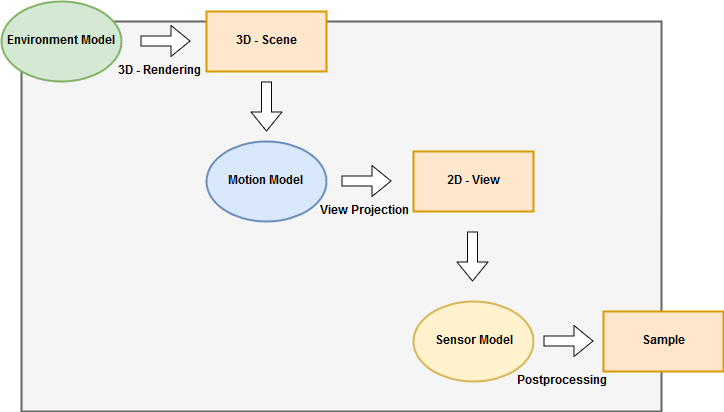
\includegraphics[width=\textwidth]{fig/Toolchain_datagen}
	\caption{Overview of the data generation process. The environment model determines background and lightning conditions and produces a 3D-Scene. The motion model determines the camera pose and location and thus the view point. Projecting the 3D-Scene on the image plane of the camera delivers the 2D-View. A final post processing step incorporates sensor and lens effects.}
	\label{fig:training:toolchain_datagen}
\end{figure}

\subsection{Scene Generation}
\label{sec:training:scene}

The first step creates a scene in which the object is embedded. Therefore it determines the context as well as light conditions.

\subsubsection{Pasting a CAD-Model on Real Images}

Inspired by \cite{Girshick2013, Peng, Rozantsev} a 3D-Model of the object of interest is pasted on real images.

The 3D-Model is provided by \todo{TODO} TODO and a tool to render these models is implemented using \textit{OpenGL}. A scene with black background is created and several objects are placed on a virtual ground plane with different rotations to each other. Additionally light sources are placed at different locations and with different intensities. 

After creating a scene the black background is replaced with an image obtained from a dataset. As the light conditions between background image and rendered scene are different, the created image can be quite artificial. Hence a post-processing step applies a Gaussian blur kernel along the edges of the CAD-model. This leads to a better embedding of the object in the background. Example outcomes can be seen in \Cref{fig:random_bg}

The parameters and locations of objects and light sources as well as the selected backgrounds can be varied when creating a dataset.

\begin{figure}[hbtp]
	\centering
	\begin{minipage}{0.49\textwidth}
		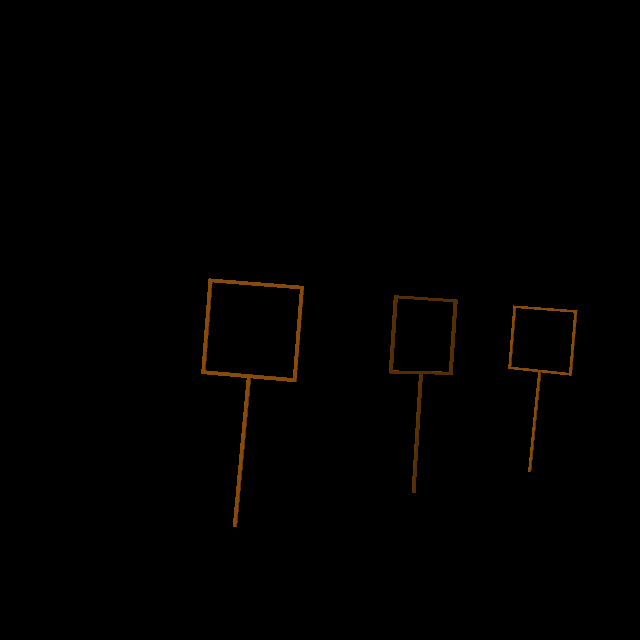
\includegraphics[width=\textwidth]{fig/shot}
	\end{minipage}
	\begin{minipage}{0.49\textwidth}
		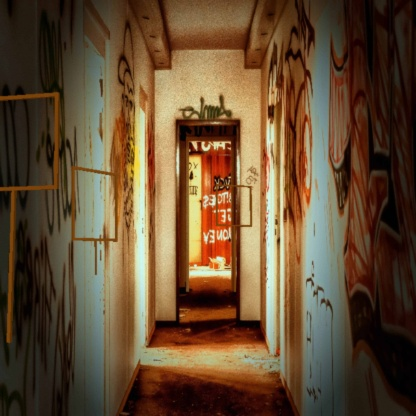
\includegraphics[width=\textwidth]{fig/random_bg2}
	\end{minipage}
	\caption{Examples for pasting the 3D-Model on various backgrounds. A scene with background is rendered (left), subsequently the black background is replaced with an image from a dataset.}
	\label{fig:random_bg}
\end{figure}

\subsubsection{Full Rendering of a Scene}

Following \cite{Ros2016, Gaidon2016, Johnson-Roberson2016, Tobin2017, Tremblay2018a} the second approach to create a scene is to fully render the environment using a graphic engine, namely the \textit{UnrealEngine} including the \textit{AirSim} plugin.

The \textit{UnrealEditor} allows to manually create environments and provides high quality rendering of objects, textures and light conditions. In total three indoor environments are created. This resembles \ac{GPS}-denied scenarios as they are targeted in this thesis. Within the environment light conditions, background textures, object locations can be changed manually.

In total three base environments are created. Examples can be seen in \Cref{fig:environments}. The three environments are described in the following:
\begin{enumerate}
	\item \textit{Basement:} The environment is a room without windows, only containing artificial light sources. 
	\item \textit{Daylight:} The environment is a room with windows along all walls that allow daylight to illuminate the room. The windows can lead to strong variations in the contrast between different parts of the object.
	\item \textit{IROS2018:} The environment resembles the room of the \ac{IROS} Autonomous Drone Race 2018. The light sources stem from a window front at one side of the room, as well as artificial light sources at the ceiling. Depending on the view point, the object might appear against bright or dark background.
\end{enumerate}

\begin{figure}[hbtp]
	\centering
	\begin{minipage}{0.49\textwidth}
		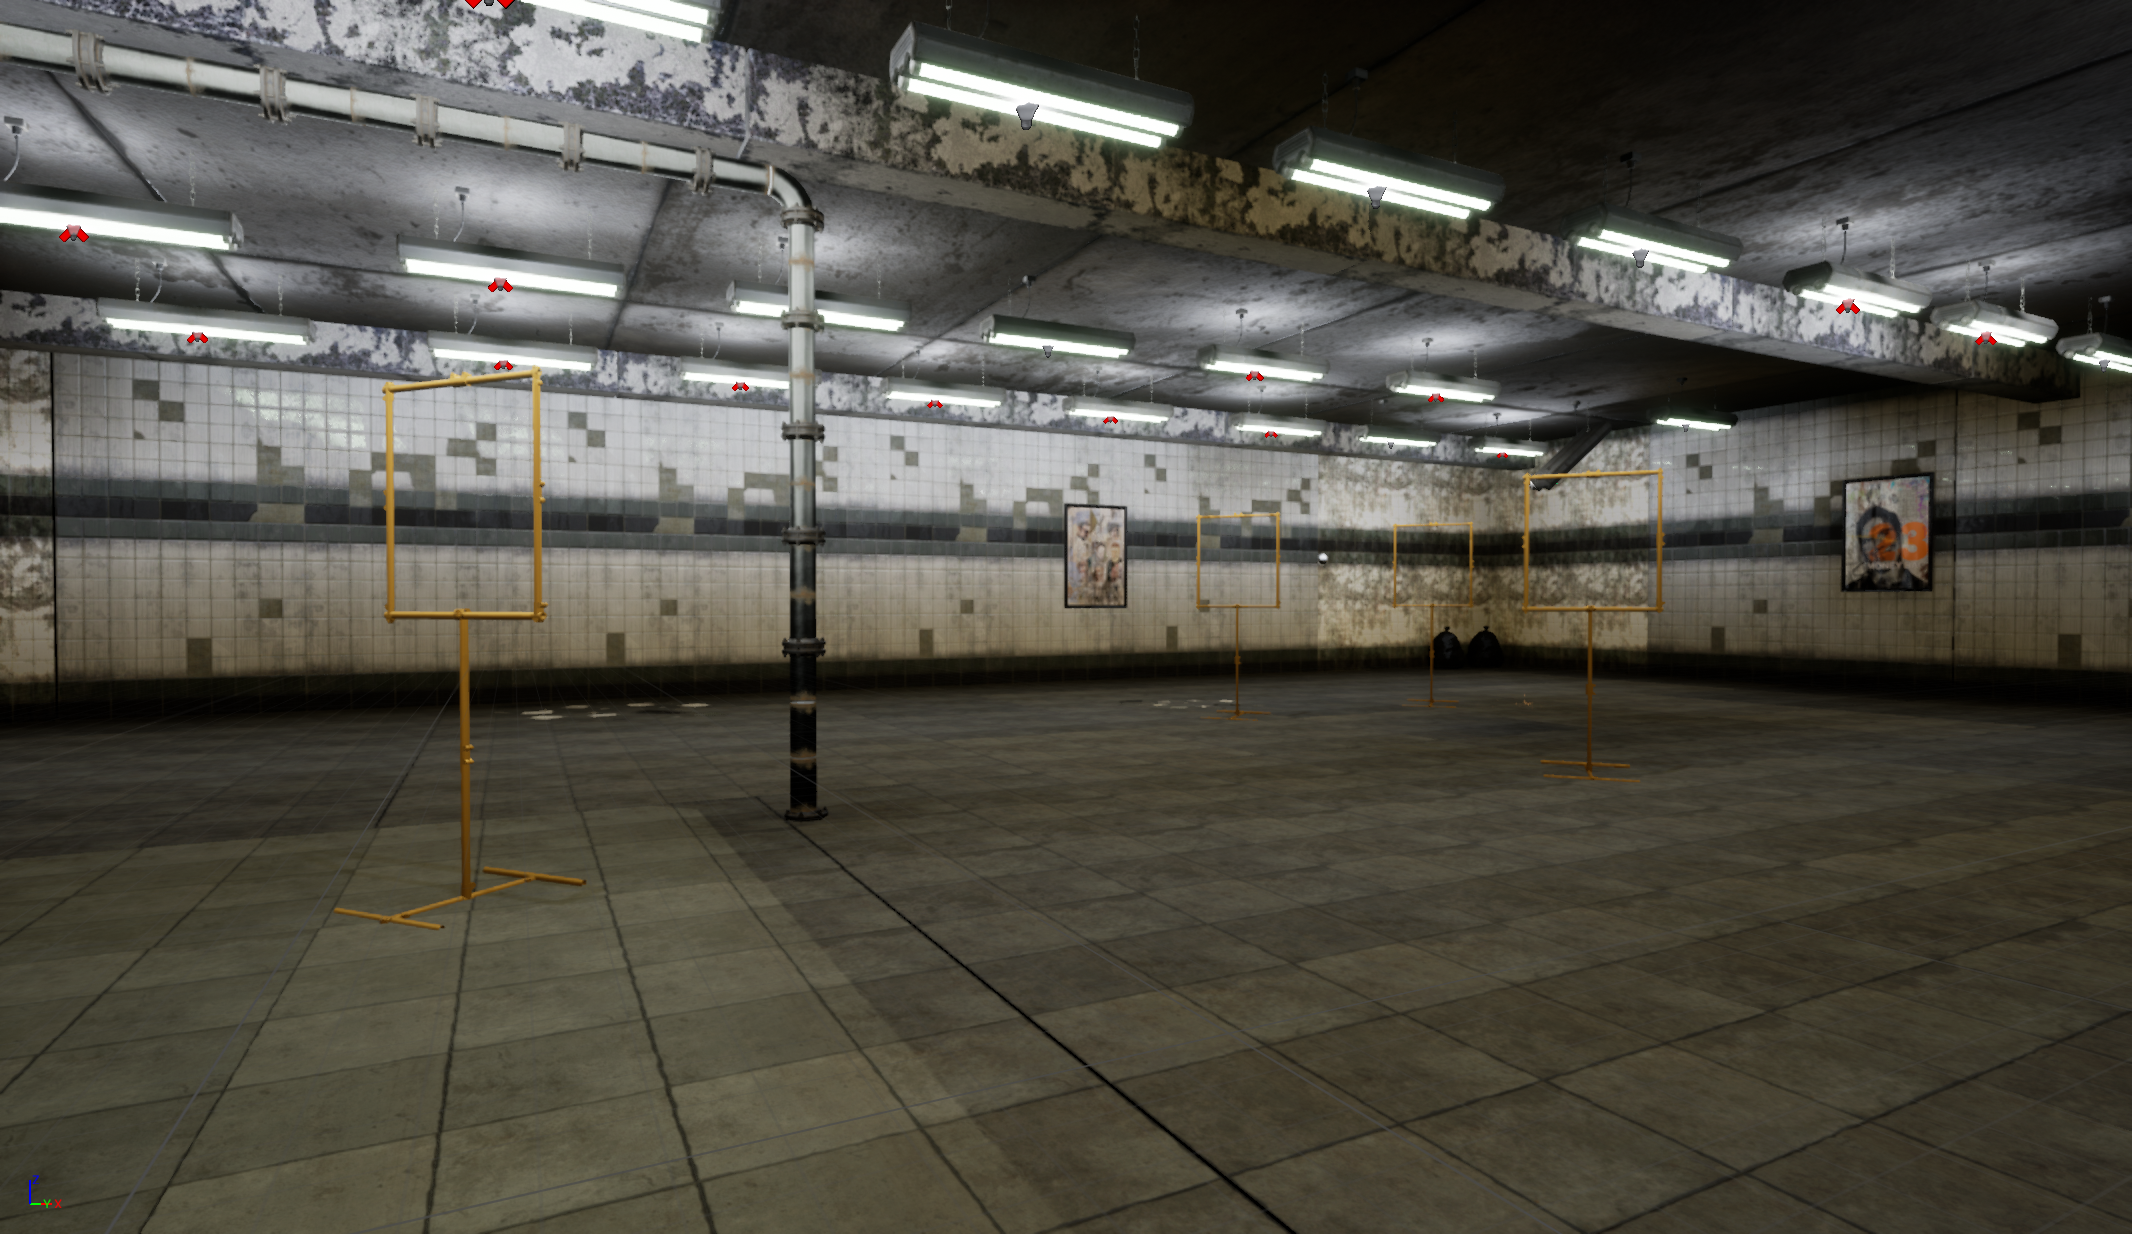
\includegraphics[width=\textwidth]{fig/basement_perspective}
	\end{minipage}
	\begin{minipage}{0.49\textwidth}
	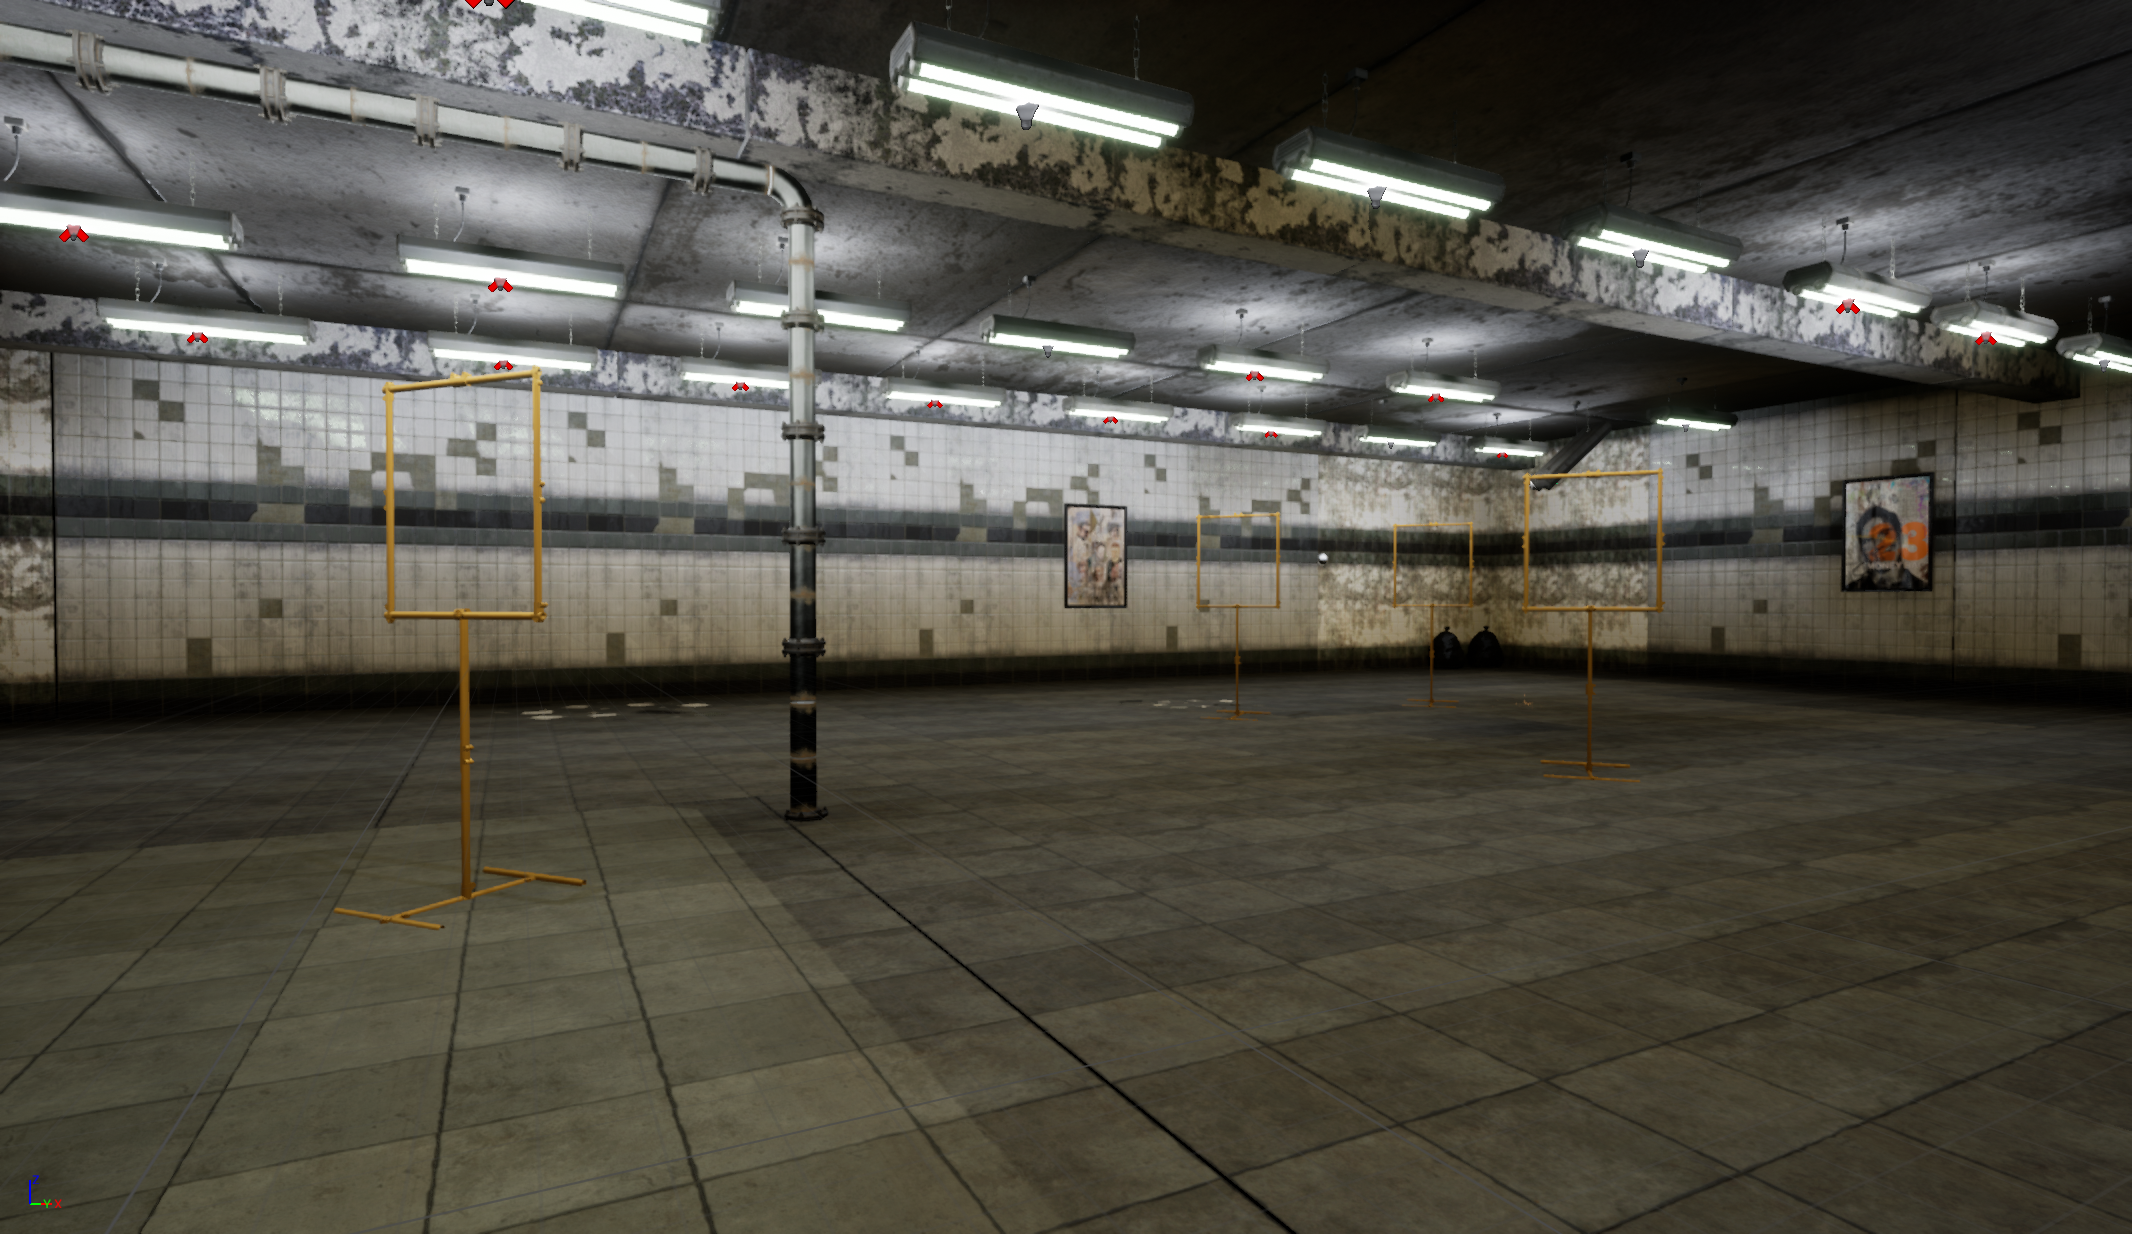
\includegraphics[width=\textwidth]{fig/basement_perspective}
\end{minipage}

\begin{minipage}{0.49\textwidth}
	\includegraphics[width=\textwidth]{fig/daylight_perspective}
\end{minipage}
\begin{minipage}{0.49\textwidth}
	\includegraphics[width=\textwidth]{fig/daylight_perspective}
\end{minipage}

\begin{minipage}{0.49\textwidth}
	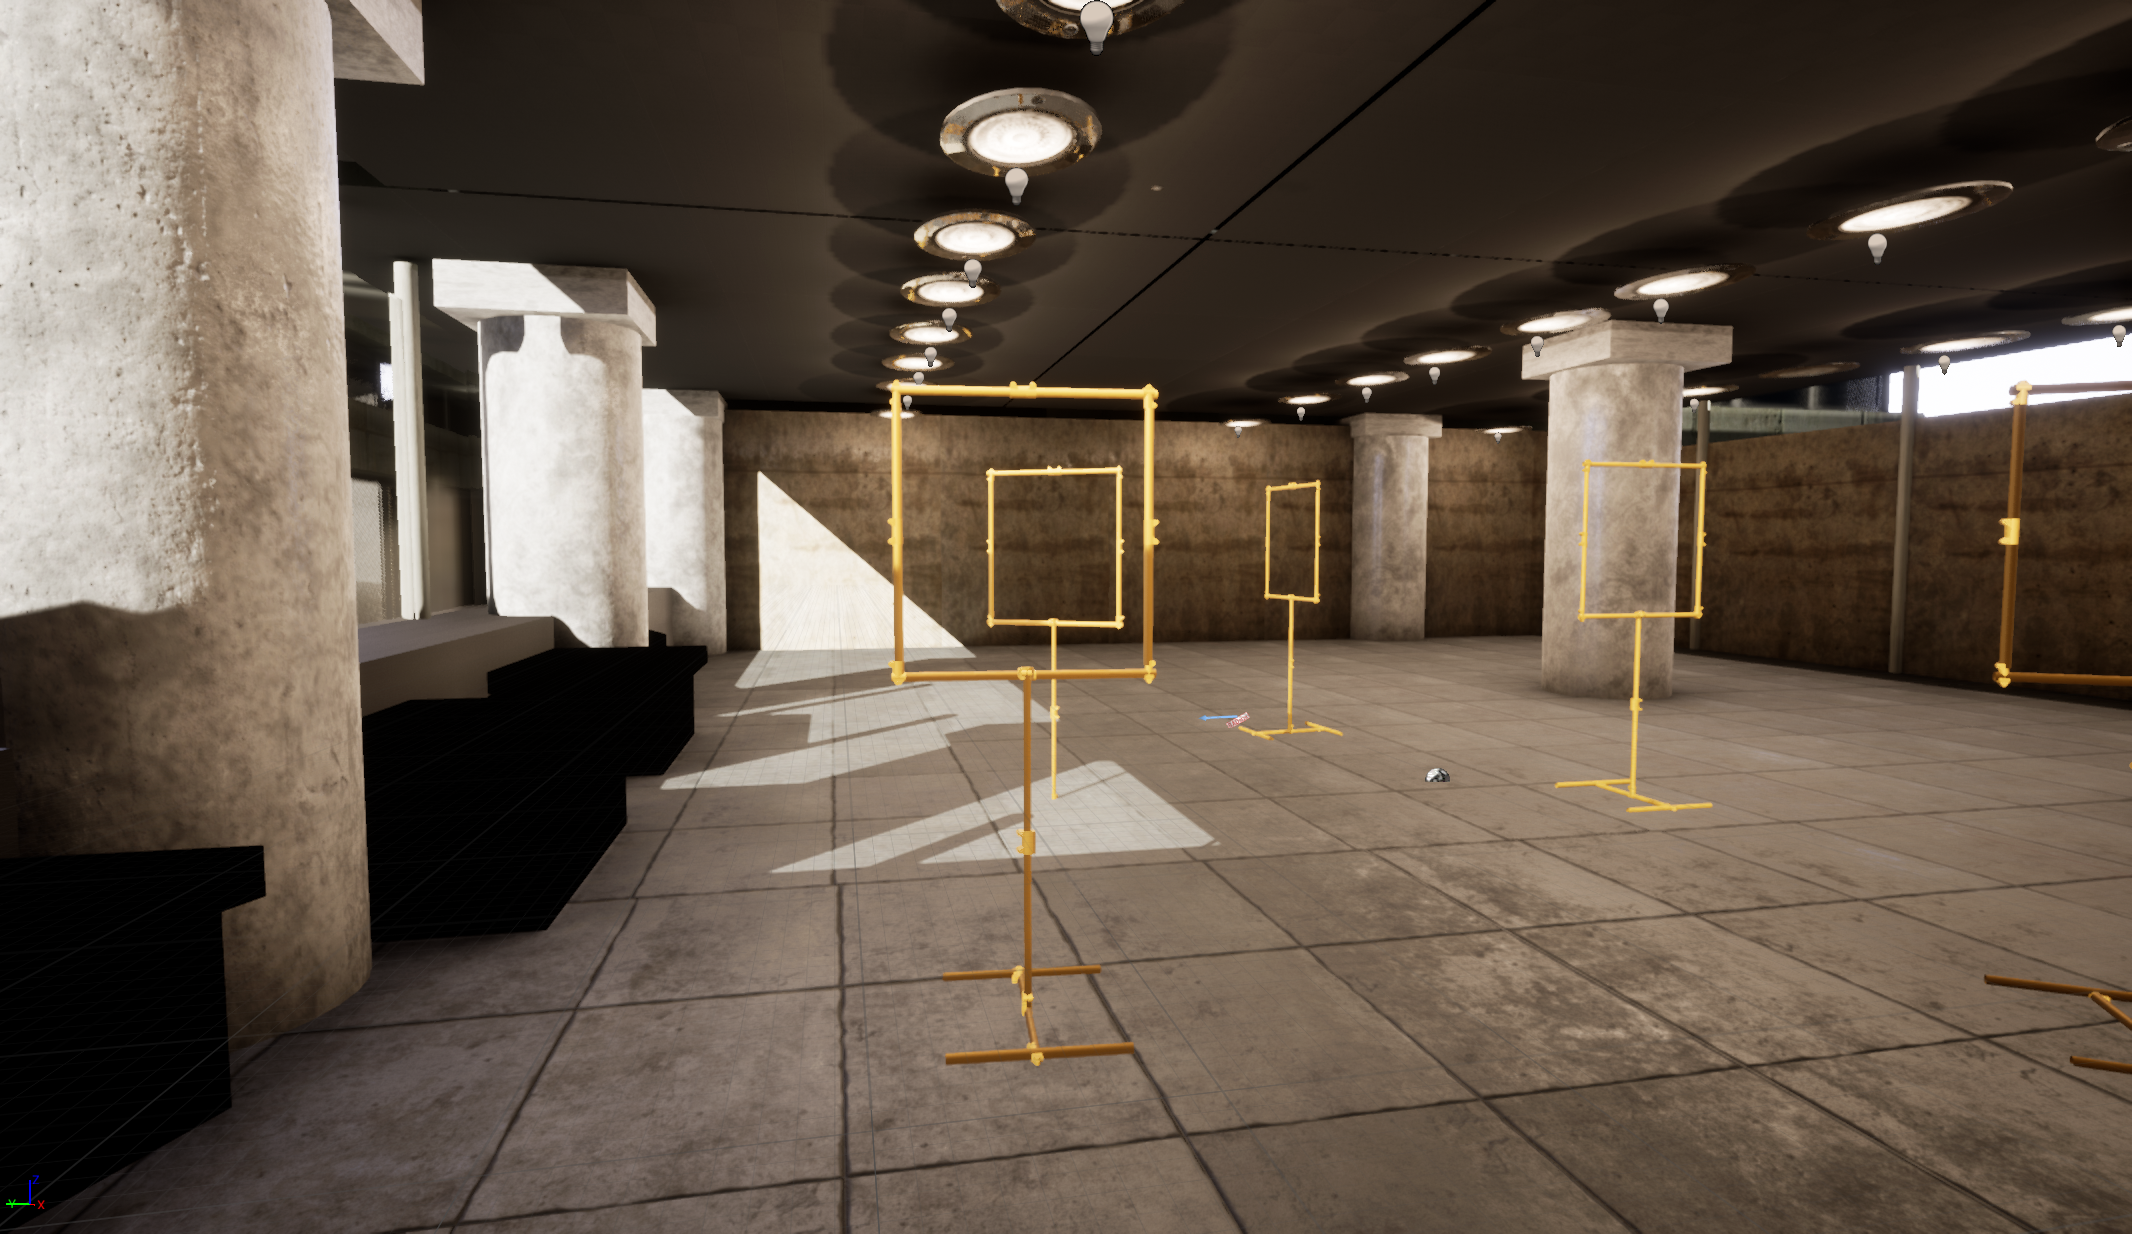
\includegraphics[width=\textwidth]{fig/iros_perspective}
\end{minipage}
\begin{minipage}{0.49\textwidth}
	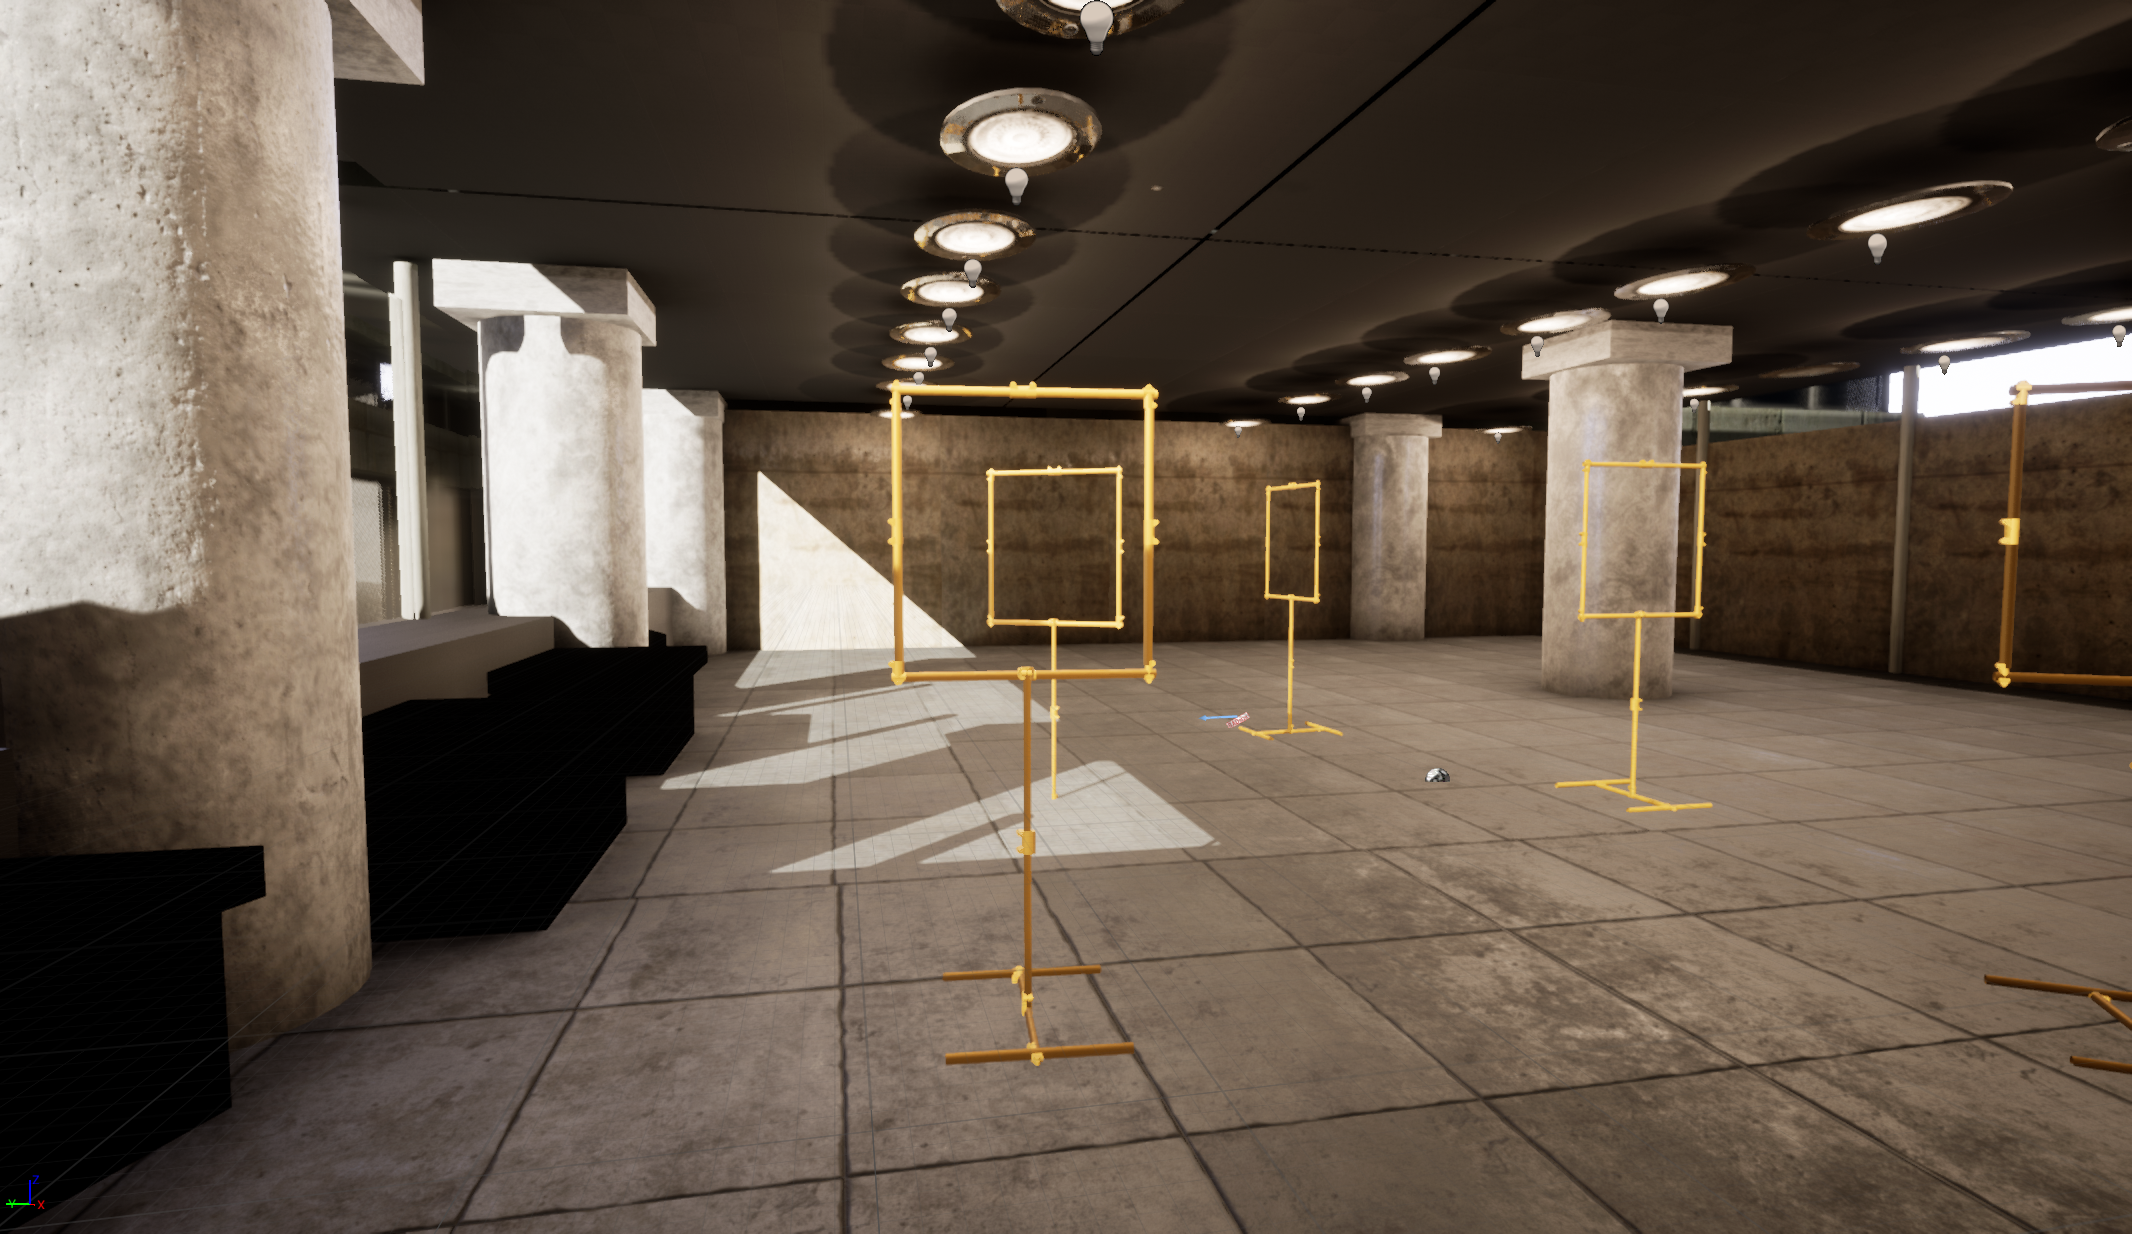
\includegraphics[width=\textwidth]{fig/iros_perspective}
\end{minipage}
\caption{Base environments when rendering a full scene. From top to bottom: \textit{Basement}, \textit{Daylight}, \textit{IROS}.}
\label{fig:environments}
\end{figure}

\subsection{Camera Placement}

The second step places the camera in the scene and creates a 2D-image. Hence, it determines the perspective of the image on the scene. The camera pose is determined by:

$$
\text{Translation: }t = [x y z] \text{ and Rotation: } r = [\phi, \theta, \psi]
$$
Where the \ac{NED} coordinate system is used originating from the initial position of the camera. 

\subsubsection{Random Placement}
	
A straightforward way of placing the camera is the random placement in the scene. The value for each dimension of $r$ and $t$ are drawn from a probability distribution. The chosen distributions have to follow certain limitations, for example the gate should still be visible in most images.
	
\subsubsection{Quad-rotor Model}
	
$r$ and $t$ follow the motion model of a quad-rotor \ac{MAV}.  The development of this model has not been done within this thesis but is summarized here for completeness: \todo{put shuos model here}.

Using this motion model, the camera follows a certain trajectory through the 3D-Environment. Storing the current image at a frequency of 2 Hz creates the corresponding samples.
	
\subsection{Post-processing}

In the final step low-level image transformations are applied. The studied methods can be distinguished in sensor model based augmentation and artificial augmentation. \comm{what do you mean by : distinguish??}

\subsubsection{Model-based augmentation}

The applied pipeline is strongly based on \cite{Carlson2018}. However, on the camera of the \ac{MAV} we assume that the raw image signal can be processed. Hence, the model for information loss due to post-processing is not included. Instead all images are converted into YUYV-colour space, a format that is obtained from most visual sensors as well as the target platform of this thesis. The pipeline is extended by two models: (1) A model for lens distortion since \ac{MAV} often use wide angle lenses to increase their \ac{FoV}; (2) A model for motion blur since fast camera movements are to be expected.

The post-processing pipeline is summarized as:

\begin{equation}
	I' = \phi_{noise}(\phi_{exposure}(\phi_{FocusBlur}(\phi_{MotionBlur}(\phi_{Chrom.}(\phi_{Lense}(I))))))
	\label{eq:postprocess}
\end{equation}

The individual models are described in the following.

\paragraph{Lens Distortion}

Lens distortion is a form of optical aberration which causes light to not fall in a single point but a region of space. For \acp{MAV} commonly used wide-angle lenses, this leads to barrel distortion and thus to straight lines appearing as curves in the image.

The effect is applied using the model for wide-angle lenses from \cite{Vass}. It models the removal of lens distortion as combination of radial and non-radial part, that is approximated with a second order Taylor expansion:

\begin{equation}
\begin{pmatrix}
	p_x' \\
	p_y'
\end{pmatrix} = \begin{pmatrix}
p_x(1 + \kappa_1 p_x^2 + \kappa_1 (1 + \lambda _x)p_y^2 + \kappa_2(p_x^2 + p_y^2)^2) \\
p_y(1 + \kappa_1 p_x^2 + \kappa_1 (1 + \lambda _y)p_y^2 + \kappa_2(p_x^2 + p_y^2)^2)
\end{pmatrix} 
\label{eq:distortion}
\end{equation}
Where:
\begin{itemize}
	\item $p_x'$ and $p_y'$ are the undistorted coordinates.
	\item $\kappa_1$ controls the primary distortion (default 0)
	\item $\kappa_2$ controls the secondary distortion (default 0)
	\item $\lambda_x$ and $\lambda_y$ controls asymmetric distortion (default 0)
\end{itemize}
 
Applying the lens distortion to an image is done using the inverse of \Cref{eq:distortion}. However, as there is no closed form solution, sthe Newton-approximation is used:

\begin{equation}
	p_i = p_{i-1} - \nabla p^{-1} (f(p)_i-p')
\end{equation}

Where $f$ is the function defined in \Cref{eq:distortion}. 

In \Cref{fig:distortion} an example is shown. The distortion is applied on the original image (left) using $k_1=0.8, k_2=0$ for the radial and non-radial part. As the distortion leads to an increased \ac{FoV}, this creates black borders in the image. Therefore the center image part is cropped and rescaled to the original image size. The right image shows the same image after the crop and rescale operation without the distortion. Thus we see the original scene (left), one possible view on that scene with a wide-angle lens (center) and the same view without the lens (right). 



\paragraph{Chromatic Aberration.}

Chromatic Aberration is caused when different wavelengths of light end up in different locations of the visual sensor. This leads to a shift in the colour channels of the image.

Similarly to \cite{Carlson2018}, chromatic aberration is applied by scaling the locations of the green channel, as well as applying translations on all channels. The model can be implemented as affine transformation of the pixel locations for each channel:

\begin{equation}
\begin{pmatrix}
x' \\
y' \\
1
\end{pmatrix} = \begin{pmatrix}
S & 0 & t_x \\
0 & S & t_y \\
0 & 0 & 1
\end{pmatrix} \begin{pmatrix}
x \\
y \\
1
\end{pmatrix}
\end{equation}

\paragraph{Motion Noise.}

Motion noise is caused when light falls in different locations of the images sensor due to a fast movement of the camera. It leads to blurry images based on the sensor motion.

The phenomenon depends on camera properties as well as the motion of camera and objects. Although a full modelling of this process might benefit the learning process, it requires a complex pipeline and is computationally expensive. Therefore a strong simplification is used, namely a one-dimensional Gaussian filter:

\begin{equation}
K_v = \begin{pmatrix}
...				 \\
\mathcal{N}(\mu-1) \\
\mathcal{N}(\mu)  \\
\mathcal{N}(\mu+1)	 \\
	...					
\end{pmatrix} \quad
K_h = \begin{pmatrix}
...	& \mathcal{N}(\mu-1)	&	\mathcal{N}(\mu) &	\mathcal{N}(\mu+1) & ...\\
\end{pmatrix}
	\label{eq:motion_noise}
\end{equation}

Where $\mathcal{N}$ is a Gaussian-PDF with mean $\mu$ and variance $\sigma$,  $K_v$ models vertical motion blur, $K_h$ horizontal motion blur. The size of the kernel is chosen by $k$.

\paragraph{Out-of-focus Blur.}

Next to motion, sensor noise can lead to blurry images. For the blur operation a 2D Gaussian kernel is applied on the input image with:

\begin{equation}
 k = \frac{1}{2\sigma_x\sigma_y\pi}e^{-\sqrt{\frac{x^2 + y^2}{2\sigma_x\sigma_y}}} 
\end{equation}

\paragraph{Exposure.}

Exposure is the time the sensor records light in order to create an image. Over- and Underexposure are caused when this time is too short or too long, leading to too dark or too bright images.

Following the model from \cite{Carlson2018}:
 
\begin{equation}
 I = f(S) = \frac{255}{1 + e^{-A S}}
\end{equation}
where $A$ is a constant term for contrast and $S$ the exposure.

The image can be re-exposed with:

\begin{equation}
	I' = f(S+\Delta S)
\end{equation}

where $S$ is obtained from :
\begin{equation}
S = f^{-1}(I) = \frac{\ln(\frac{255}{I}-1)}{-A}
\end{equation}

\paragraph{Noise.}
\todo{text}

\subsection{Artificial Augmentation}

Inspired by \cite{Howard2013, Redmon, Liu} the application of several artificial image transformations is studied. The overall goal is to generate more variations in the input signal and thus to make the model more invariant against changes in those properties. We do not use image scaling or translation for augmentation as it is easier to incorporate such variations using the motion model.

\paragraph{Brightness.} In order to obtain a model that is more robust against illumination changes image brightness is alternated. Therefore a scaling on the V-channel in HSV-colour space is applied. The scaling is drawn from a uniform distribution.
	
\paragraph{Grayscale.} By transforming a subset of samples into grayscale images, the model is forced to learn more color invariant features. 
	
\paragraph{Histogram Equalization.} Changes in the environmental conditions can also affect contrast. By applying a histogram equalization on a subset of images, variations in contrast are achieved. \todo{describe}
	
\paragraph{Flip.} By mirroring the image vertically, more variations in object locations are achieved. The operation is applied with a probability of $f$.


\begin{figure}[htbp]
	\centering
	\begin{minipage}{0.49\textwidth}
		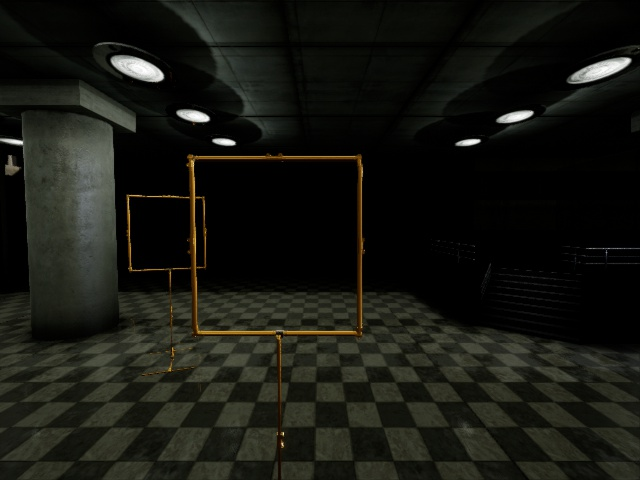
\includegraphics[width=\textwidth]{fig/gate_example}
	\end{minipage}
	\begin{minipage}{0.49\textwidth}
		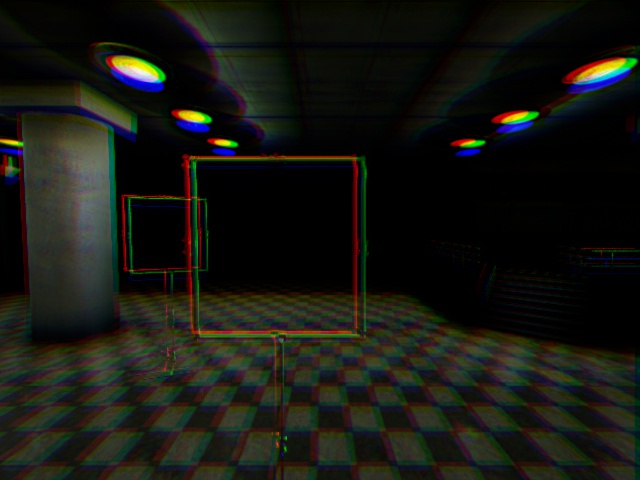
\includegraphics[width=\textwidth]{fig/gate_example_chromatic}
	\end{minipage}
	\caption{Example Chromatic Aberration with $S=[1, 1.01, -5.0]$, $t_x=[10,0.1,0.01]$, $t_y=[0.1,-0.1,0.0.01]$. Original scene (left), after transformation (right)}
	\label{fig:chromatic}
\end{figure}
\begin{figure}[htbp]
	\begin{minipage}{0.33\textwidth}
		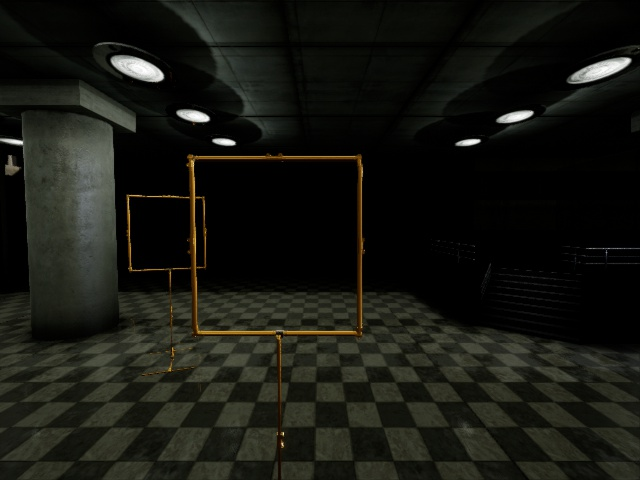
\includegraphics[width=\textwidth]{fig/gate_example}
	\end{minipage}
	\begin{minipage}{0.33\textwidth}
		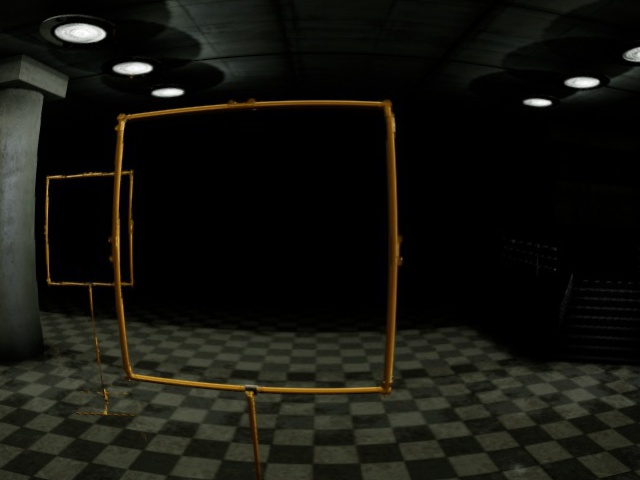
\includegraphics[width=\textwidth]{fig/gate_example_distorted}
	\end{minipage}
	\begin{minipage}{0.33\textwidth}
		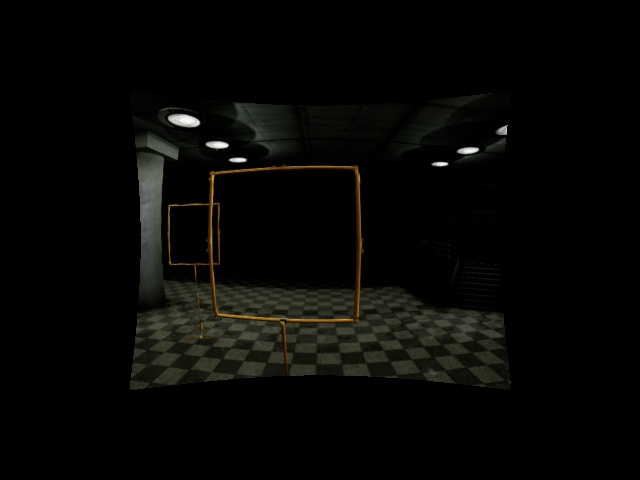
\includegraphics[width=\textwidth]{fig/gate_example_undistorted}
	\end{minipage}
	\caption{Example Lens Distortion. Original scene (left), distorted view (center), undistorted view (right)}
	\label{fig:distortion}
\end{figure}

\begin{figure}[htbp]
	\centering
	\begin{minipage}{0.49\textwidth}
		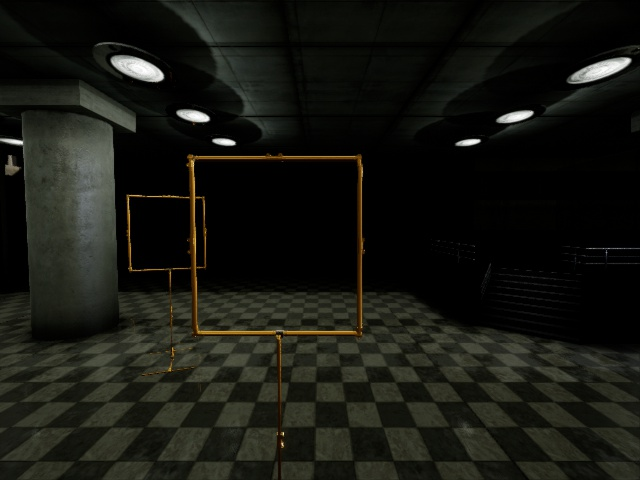
\includegraphics[width=\textwidth]{fig/gate_example}
	\end{minipage}
	\begin{minipage}{0.49\textwidth}
		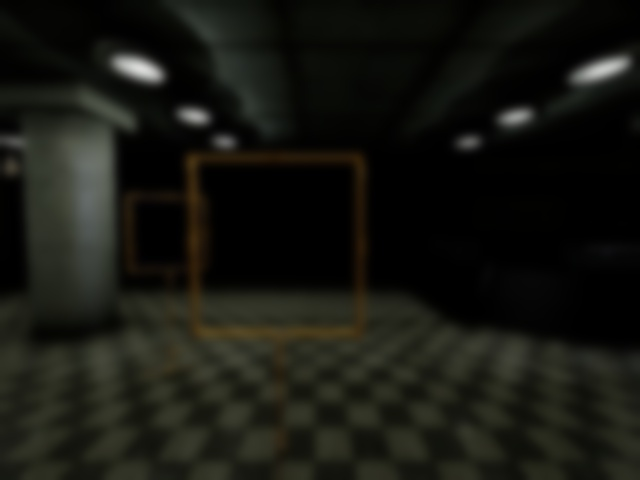
\includegraphics[width=\textwidth]{fig/gate_example_focusblur}
	\end{minipage}
	\caption{Example Out-of-Focus blur.}
	\label{fig:focusblur}
\end{figure}

\begin{figure}[htbp]
	\begin{minipage}{0.33\textwidth}
		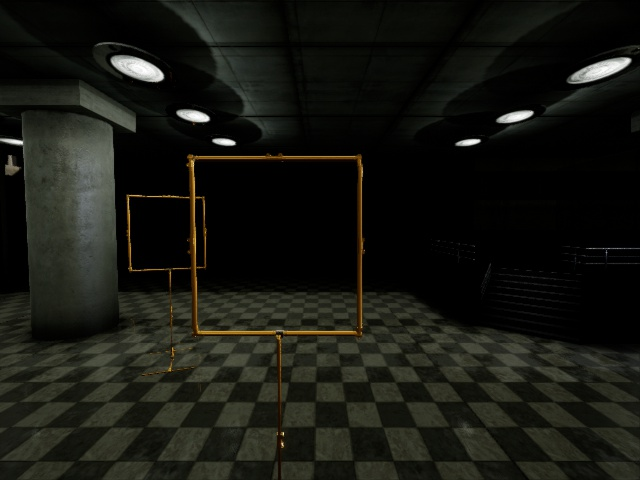
\includegraphics[width=\textwidth]{fig/gate_example}
	\end{minipage}
	\begin{minipage}{0.33\textwidth}
		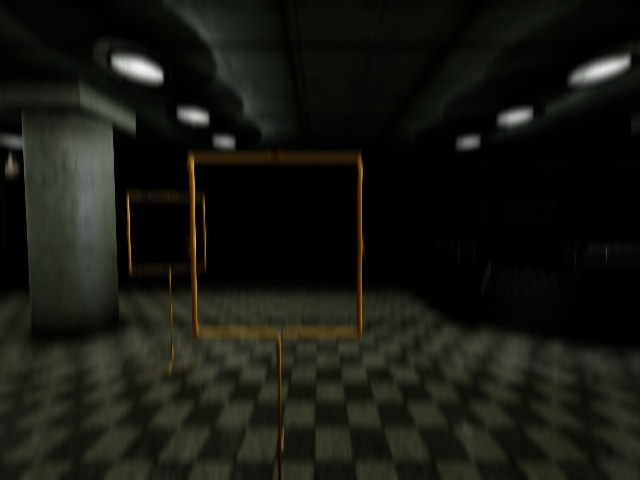
\includegraphics[width=\textwidth]{fig/gate_example_motionblur_v}
	\end{minipage}
	\begin{minipage}{0.33\textwidth}
		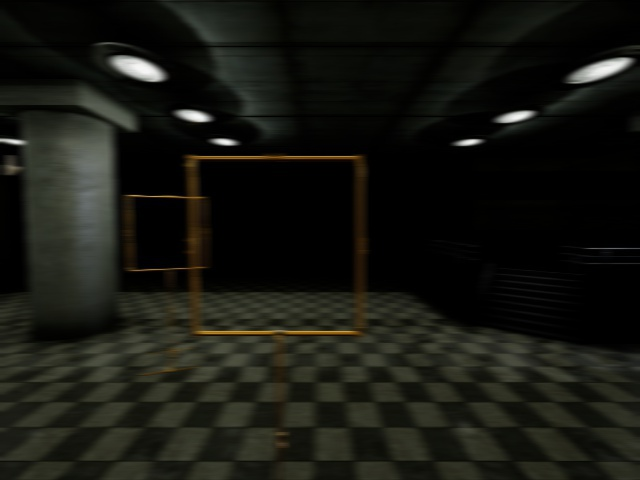
\includegraphics[width=\textwidth]{fig/gate_example_motionblur_h}
	\end{minipage}
	\caption{Example Motion Blur with $k=15$, $\sigma=5.0$. Original scene (left), vertical movement (center), horizontal movement (right)}
	\label{fig:motionblur}
\end{figure}

\begin{figure}[htbp]
	\centering
	\begin{minipage}{0.49\textwidth}
		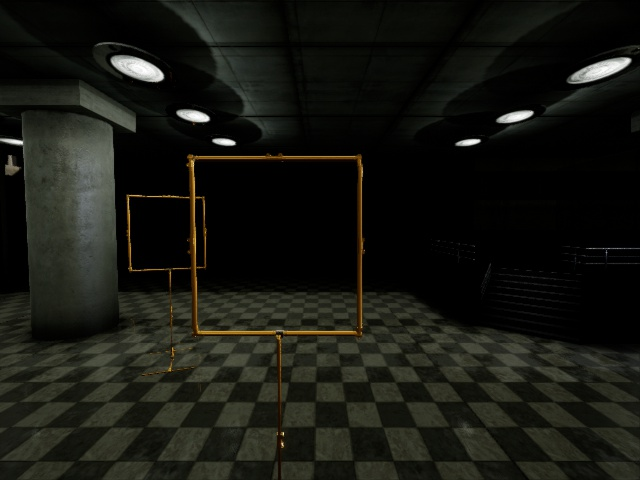
\includegraphics[width=\textwidth]{fig/gate_example}
	\end{minipage}
	\begin{minipage}{0.49\textwidth}
		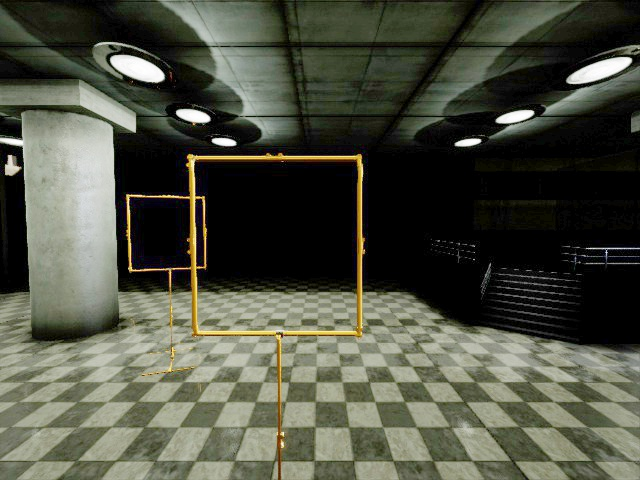
\includegraphics[width=\textwidth]{fig/gate_example_exposure}
	\end{minipage}
	\caption{Example Exposure with $\Delta S = 2.0$, $A = 1.0$.}
	\label{fig:exposure}
\end{figure}

\subsection{Hypothesis}
\label{sec:training:hypothesis}

Most of described approaches in \Cref{sec:training:related} focus on objects that have complex structures and therefore provide robust features that are independent of the rest of the scene. For example a face contains eyes and a nose, whose appearances are influenced to some extent by light conditions but relatively independent from image background. It has been shown in \todoref{visualizing cnns} how object detectors exploit this kind of structure in the learned representation. We hypothesize that a model to detect such complex objects is less domain dependent and can therefore be more easily transferred to domains with other environmental conditions. That is the performance drop $\Delta m$ of a model trained in $S$ and applied in $T$ where $S$ and $T$ are different in terms of environmental conditions will be larger for an \ac{EWFO} than for a more complex object.

If the environmental conditions have an high impact, their modelling is particularly important in the data generation process. We hypothesize that, as pasting the image on random backgrounds fails to capture these conditions, it is not a sufficient method to train a model for the detection of \acp{EWFO}. That is the performance drop $\Delta m$ of a model trained in $S$ and applied in $T$ where $S$ is generated by pasting a 3D-Mesh on random backgrounds and $T$ is modelled using full environment rendering will be prohibitively large.
 
From that it follows that in order to generate data for \ac{EWFO} Object Detection it is particularly important to address the domain shift. In literature two ways to approach this problem on the data level can be found: (1) providing a lot of variance in the training data to obtain a representation that is robust against domain shifts; (2) including target domain knowledge in the training data to obtain a representation that is tailored to the target domain. We hypothesize that there is a trade-off between these two approaches: a model that performs well across domains will perform poorer in a particular domain but better in other domains compared to a model that is trained for that particular domain. Hence, we hypothesize, if knowledge of $T$ is included when generating $S$ the performance in $T$ will improve given a fixed modelsize/ the model can be simplified achieving equal performance. \comm{what??}

In the data generation process this can be addressed on several levels:

\begin{enumerate}
	\item \textbf{Scene Generation.} A model trained for a particular room, with particular lightning conditions will perform better in that room but perform poorly in other rooms than a model trained on various rooms with various lightning conditions. By modelling the environment of the real data, the performance on the real data can be improved.
	
	\item \textbf{Camera Placement.} A model trained using the quad-rotor model will perform better on real data than a model trained using random camera locations.
	
	\item \textbf{Postprocessing.} A model trained using a post-processing pipeline that models the real-world sensor will perform better on the real data than a model that is trained on using varying parameters in the post-processing pipeline.  
\end{enumerate}

The hypotheses are summarized in the following:

\begin{enumerate}
	\item[$\mathcal{H}_1$] The performance drop $\Delta m$ of a model trained in $S$ and applied in $T$ where $S$ and $T$ are different in terms of environmental conditions will be larger for an \ac{EWFO} than for a more complex object.
	
	\item[$\mathcal{H}_2$] In contrast to a more complex object, the performance drop $\Delta m$ of a model for the detection of \acp{EWFO} trained in $S$ and applied in $T$ where $S$ is generated by pasting a 3D-Mesh on random backgrounds and $T$ is modelled using full environment rendering will be prohibitively large.
	
	\item[$\mathcal{H}_3$] A model trained in $S_0$ where $S_0 \in S$ and applied in $T_0$, where $S_0 = T_0$ will perform better in $T_0$ than a model that is trained in $S$ but perform worse in $T_1$ where $T_1 \in S$ and $T_1 \neq S_0$. 

	\item[$\mathcal{H}_3$] By including properties of $T$ in $S$ where $S$ is an artificial set $T$ is the real data, the performance $m_T$ of a model can be improved. 

\end{enumerate}

\section{Experiments}
\label{sec:training:experiments}
In order to evaluate the formulated hypotheses several experiments are conducted. The model used is the TinyYoloV3-Architecture, further described in \Cref{sec:object_detection}.\comm{missing thing???} The reported metrics are described in \Cref{sec:metrics}. For all experiments mean and standard deviation of 10 runs are reported.
\begin{equation}
	x = \mathcal{U}(-30,30),\quad y = \mathcal{U}(-20,20),\quad z = \mathcal{N}(-4.5,0.5)),\quad
	\phi = \mathcal{U}(0,0.1\pi),\quad \theta = \mathcal{U}(0,0.1\pi),\quad \psi = \mathcal{N}(-\pi,\pi)
	\label{eq:distroexp}
\end{equation}


\subsection{Experiment I}

In order to evaluate $\mathcal{H}_1$ a model is trained in $S$ and applied in $T$. Three objects are investigated namely the \textit{Square-Gate}, \textit{Round-Gate} and \textit{Person.} The source environment is \textit{Basement}, the target domain is \textit{Daylight.} The training set consists of 20 000 samples, where for every batch of 2000 samples the objects are rearranged in the room. The test set consists of 1000 samples and fixed object arrangement. The view points are samples from the distributions described in the following:
$$
x = \mathcal{U}(-30,30),\quad y = \mathcal{U}(-20,20),\quad z = \mathcal{N}(-4.5,0.5)
$$
$$
\phi = \mathcal{U}(0,0.1\pi),\quad \theta = \mathcal{U}(0,0.1\pi),\quad \psi = \mathcal{N}(-\pi,\pi)
$$
Where $ \mathcal{U}(a,b)$ is a uniform distribution between $a,b$ and $\mathcal{N}(\mu,\sigma^2)$ is a Gaussian distribution with mean $\mu$ and variance $\sigma^2$.
The parameters are chosen experimentally aiming to resemble common view points of a person standing in the room.


\subsection{Experiment II}

In order to evaluate $\mathcal{H}_2$ a model is trained in $S$ and applied in $T$. Three objects are investigated namely the \textit{Square-Gate}, \textit{Round-Gate} and \textit{Person.}  The training set consists of 20 000 samples, where for every batch of 2000 samples the objects are rearranged in the room. The test set consists of 1000 samples and fixed object arrangement. The training set is generated by replacing the background with images samples from the Pascal VOC dataset. The test set is taken in \textit{Daylight} Environment. The view points are samples from the distributions described in the following:

Where $ \mathcal{U}(a,b)$ is a uniform distribution between $a,b$ and $\mathcal{N}(\mu,\sigma^2)$ is a Gaussian distribution with mean $\mu$ and variance $\sigma^2$.
The parameters are chosen experimentally aiming to resemble common view points of a person standing in the room.

\subsection{Experiment III}

In order to evaluate $\mathcal{H}_3$ the individual domain properties and their incorporation in the data generation process are studied. Each property is compared in terms of specialization and generalization. That is the property are varied between three configurations: (1) resembling the target domain, (2) generalizing across domains, (3) disabled (if applicable).

The test set is generated in the environment \textit{IROS}, using the quad-rotor model. In total 1000 images are sampled taken from one trajectory. The post-processing applies:
\begin{enumerate}
	\item Lense distortion
	\item Chromatic Abberration
	\item Motion Blur
	\item Out-of-Focus Blur
	\item Exposure
\end{enumerate}

\subsection{Experiment IV}

In order to evaluate $\mathcal{H}_4$ the individual domain properties are measured on the target domain and incorporated in the training set.


\section{Results}
\label{sec:training:results}

\section{Discussion}
\label{sec:training:discussion}

\section{Conclusion}
\label{sec:training:conclusion}


